\documentclass[letterpaper,9pt,twocolumn,twoside,]{pinp}

%% Some pieces required from the pandoc template
\providecommand{\tightlist}{%
  \setlength{\itemsep}{0pt}\setlength{\parskip}{0pt}}

% Use the lineno option to display guide line numbers if required.
% Note that the use of elements such as single-column equations
% may affect the guide line number alignment.

\usepackage[T1]{fontenc}
\usepackage[utf8]{inputenc}

% pinp change: the geometry package layout settings need to be set here, not in pinp.cls
\geometry{layoutsize={0.95588\paperwidth,0.98864\paperheight},%
  layouthoffset=0.02206\paperwidth, layoutvoffset=0.00568\paperheight}

\definecolor{pinpblue}{HTML}{185FAF}  % imagecolorpicker on blue for new R logo
\definecolor{pnasbluetext}{RGB}{101,0,0} %



\title{The variables which affect the academic success of a student}

\author[]{Sura Majeed}
\author[]{Junhao Liu}
\author[]{Elena Skorokhodova}
\author[]{Mason Wong}
\author[]{Hoang Dao}

  \affil[]{University of Sydney}

\setcounter{secnumdepth}{0}

% Please give the surname of the lead author for the running footer
\leadauthor{}

% Keywords are not mandatory, but authors are strongly encouraged to provide them. If provided, please include two to five keywords, separated by the pipe symbol, e.g:
 

\begin{abstract}
This report analyses students' performance in Portuguese using
statistical methods to understand relevant factors that affect students'
final grades. The report aims to help students and school faculty
understand which factors can be changed to predict and improve student
performance. The dataset was analysed using multiple linear regression
and various model selection approaches to obtain the best model. The
optimal model found that various social and familial factors could
heavily influence student performance. Schools can apply these results
by understanding and targeting the factors found to affect students'
failure rates.
\end{abstract}

\dates{This version was compiled on \today} 


% initially we use doi so keep for backwards compatibility
% new name is doi_footer


\begin{document}

% Optional adjustment to line up main text (after abstract) of first page with line numbers, when using both lineno and twocolumn options.
% You should only change this length when you've finalised the article contents.
\verticaladjustment{-2pt}

\maketitle
\thispagestyle{firststyle}
\ifthenelse{\boolean{shortarticle}}{\ifthenelse{\boolean{singlecolumn}}{\abscontentformatted}{\abscontent}}{}

% If your first paragraph (i.e. with the \dropcap) contains a list environment (quote, quotation, theorem, definition, enumerate, itemize...), the line after the list may have some extra indentation. If this is the case, add \parshape=0 to the end of the list environment.


\hypertarget{introduction}{%
\subsection{Introduction}\label{introduction}}

A student's performance is not only affected by intelligence or effort
but also could be influenced by other factors. The Portuguese secondary
educational system faces a problem of high failure rates for students in
fundamental language courses. In an effort to investigate the system's
potential drawbacks, this report aims to examine student performance in
the Portuguese language against different demographic, social, familial
and school-related factors and find the key variables that influence
educational success. An outcome of the report would assist in a thorough
assessment of students' abilities and achievements in secondary
education, allowing the schools to improve the education quality and
target corrective measures with the overall goal to lower students' high
failure rates.

\hypertarget{data-description}{%
\subsection{Data description}\label{data-description}}

The data was obtained from 2 sources, a questionnaire with 37 closed
questions and mark reports for students from 2 Portuguese public
secondary schools.The data was collected in years 2005-2006 over the
school year and contains 649 observations. The independent variable is
the final grade (last evaluation in the school year) with a 20-point
grading scale. In the cleaning process of this data we used factor() on
the nominal categorical variables and left ordinal ones as numeric. The
reasons behind this are to maintain the importance of order in these
variables, and to simplify the interpretation (Kassambara, 2018).

\hypertarget{analysis}{%
\subsection{Analysis}\label{analysis}}

We begin with the analysis of the full model containing 30 dependent
variables. All of the variables plotted exhibited relatively linear
relationships, with the data distributed evenly around their respective
line of best fit, fulfilling the linearity assumption. Figure 1
demonstrates the linearity for 6 variables with the rest exibiting the
same pattern. The experiment was designed so that each student's
responses were a different observation. There is nothing to suggest that
these students' outcomes depend on one another; therefore, the
independence assumption is not violated.\linebreak

\begin{figure}
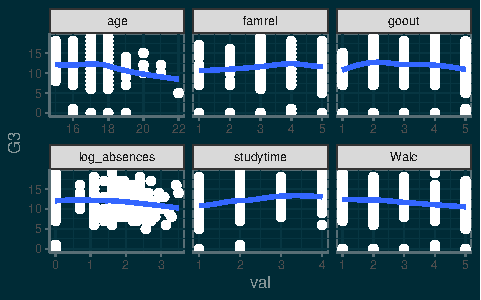
\includegraphics{report_files/figure-latex/unnamed-chunk-1-1} \caption{Checking linearity assupmtion for full model}\label{fig:unnamed-chunk-1}
\end{figure}

There does not seem to be any trends in the plot of the fitted vs
residuals; there is some concern around the bottom left but not enough
to violate the homoscedasticity assumption. Furthermore, linearity in
fitted vs residuals seems not violated. The QQ plot shows that most of
the data is close to the line except for the very bottom of the graph,
which is heavily skewed. However, the Central Limit Theorem ensures that
all inferences are still valid (Figure 2).\linebreak

\begin{figure}
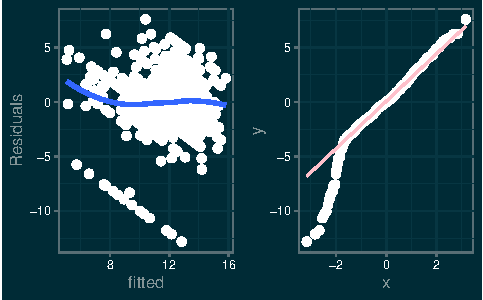
\includegraphics{report_files/figure-latex/unnamed-chunk-2-1} \caption{Checking homoscedasticity and normality assupmtions for full model}\label{fig:unnamed-chunk-2}
\end{figure}

To find the best model, first, we applied in sample approach using
backward and forward stepwise selection (Figure 3). We used the
minimisation of the AIC criterion as the most widely used method for
model selection. After forward and backward selection, we ended up with
two different models with much smaller AIC than the full
model.\linebreak 

\begin{figure}
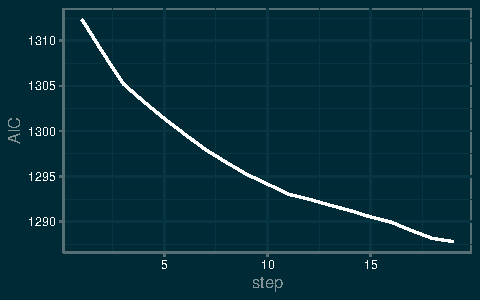
\includegraphics{report_files/figure-latex/unnamed-chunk-3-1} \caption{Backward selection using AIC minimisation}\label{fig:unnamed-chunk-3}
\end{figure}

\hypertarget{results}{%
\subsection{Results}\label{results}}

Through these comparisons, the backward model has the least AIC and the
biggest adjusted R squared value (Figure 4). Therefore, it suggests that
the backward model is better for predicting and explaining the observed
grade value. Moreover, results of the out of sample approach using
7-fold cross-validation demonstrated that RMSE and MAE are smaller for
the backward model, which increases our confidence in using this model
(Figure 5).\linebreak

\begin{figure}[h]
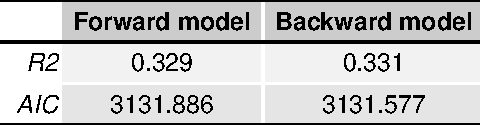
\includegraphics{report_files/figure-latex/unnamed-chunk-4-1} 
\caption{Models Summary}
\end{figure}

\begin{figure}
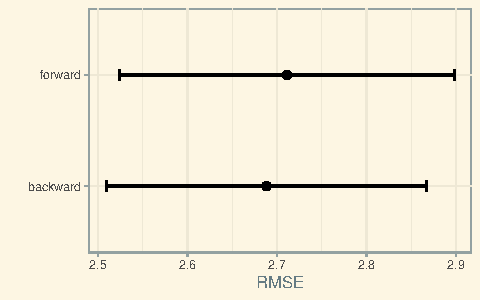
\includegraphics{report_files/figure-latex/unnamed-chunk-6-1} \caption{RMSE comparison for forward and backward models}\label{fig:unnamed-chunk-6}
\end{figure}

Checking assumptions for our final model, the residuals plot does not
seem to show any strong pattern, which indicates that neither the
linearity nor homoscedasticity assumption is violated. The QQ plot has
some concern around the lower tail, but the CLT ensures all inferences
are still valid (Figure 6). Lastly, an Anova test on the regression
showed us that all the predictors in our final model are
significant.\linebreak

\begin{figure}
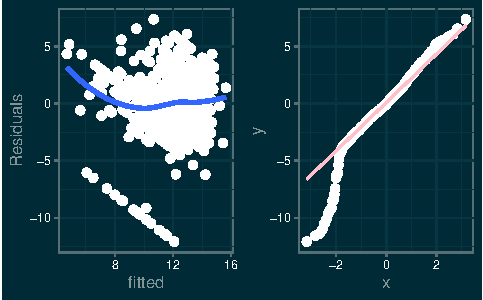
\includegraphics{report_files/figure-latex/unnamed-chunk-8-1} \caption{Checking homoscedasticity and normality assupmtions for final model}\label{fig:unnamed-chunk-8}
\end{figure}

Our final fitted model:
\(Grade = 8.84 + (-1.50) failures + (-1.43) schoolMS + (1.90) higheryew + (0.43) studytime + (-1.31) schoolsupyes + (-0.39) Dalc + (-0.17) health + (-0.55) sexM + (-0.44) romenticyes + (0.16) age + (0.30) Medu + (-0.47) guardianMother + (-0.04) guardianOther\)
\linebreak

Interpreting the most interesting estimated coefficients, we can
conclude the following. On average, holding all other variables
constant, one unit increase in the number of failures results in a 1.5
unit decrease in grade. On average, holding all other variables
constant, a level increase in mother education results in a 0.30 unit
increase in grade. On average, holding the other variables constant, if
a student wants to take higher education, there is a 1.90 unit increase
in grade. On average, holding all other variables constant, one unit
increase in health status results in a 0.17 unit decrease in grade. High
achieving students are shown to have poor health, and it is reasonable
to consider that students with higher grades get poor health because of
studying late or overstudying. Moreover, one more possible explanation
could be the very subjective nature of the answers.\linebreak

\hypertarget{discussion-and-conclusion}{%
\subsection{Discussion and conclusion}\label{discussion-and-conclusion}}

We have found that our linear model explains 31.5\% of the observed
variation in the final grade. The analysis demonstrated that past
failures are the most significant predictor similar to another research
(Cortez and Silva, 2008). Our model had great diversity in predictor
variables, including school-related, family and social variables.
\linebreak

As a result, we can conclude that other factors (social and familial)
could influence the students' academic performance and could be targeted
to decrease failure rates. For example, one of the significant
predictors was whether the student wanted to continue education or not.
So, the schools could provide more information to students about
possibilities and benefits if they continue their education. \linebreak

Finally, our project has several limitations, including linear
regression utilisation. However, more complicated methods such as random
forest or neural networks could potentially produce better results
(Cortez and Silva, 2008). Moreover, we used data on only two particular
schools, which can produce specific results. Therefore, future studies
might increase the scope of the research looking at a more diverse
school range. Lastly, there are probably interactions between the
variables which could affect the results.\linebreak

\hypertarget{github}{%
\subsection{Github}\label{github}}

The following link is the link to our github repository. Clone it and
see our work for yourselves!

\url{https://github.sydney.edu.au/jliu7095/LAB-02-CC_early_4.git}
\linebreak

\hypertarget{references}{%
\subsection{References}\label{references}}

\small

\begin{itemize}
\item
  Cortez, P., \& Silva, A. M. G., 2008, \emph{Using data mining to
  predict secondary school student performance}, viewed 20th October
  2021, \url{http://www3.dsi.uminho.pt/pcortez/student.pdf}
\item
  Kassambara, A, 2018, \emph{Regression with Categorical Variables:
  Dummy Coding Essentials in R}, viewed 22nd October 2021,
  \url{http://www.sthda.com/english/articles/40-regression-analysis/163-regression-with-categorical-variables-dummy-coding-essentials-in-r/}
\item
  R Core Team, 2021, \emph{A language and environment for statistical
  computing. R Foundation for Statistical Computing}, viewed 13th
  November 2021, \url{https://www.R-project.org/}
\item
  Wickham H, Averick M, Bryan J, Chang W, McGowan LD, François R,
  Grolemund G, Hayes A, Henry L, Hester J, Kuhn M, Pedersen TL, Miller
  E, Bache SM, Müller K, Ooms J, Robinson D, Seidel DP, Spinu V,
  Takahashi K, Vaughan D, Wilke C, Woo K, Yutani H, 2019, \emph{Welcome
  to the tidyverse}, Journal of Open Source Software, 4(43), 1686. doi:
  10.21105/joss.01686, viewed 13th November 2021
\item
  Horikoshi M, Tang Y, 2018, \emph{ggfortify: Data Visualization Tools
  for Statistical Analysis Results}, viewed 13th November 2021,
  \url{https://CRAN.R-project.org/package=ggfortify}
\item
  Wickham H, 2016, \emph{ggplot2: Elegant Graphics for Data Analysis},
  pringer-Verlag New York. ISBN 978-3-319-24277-4, viewed 13th November
  2021, \url{https://ggplot2.tidyverse.org}
\item
  Kuhn, M. 2008, \emph{Building Predictive Models in R Using the caret
  Package}, Journal of Statistical Software, 28(5), 1 - 26. doi, viewed
  on 13th November 2021, \url{http://dx.doi.org/10.18637/jss.v028.i05}
\item
  Xie, Y. 2015, \emph{Dynamic Documents with R and knitr}, 2nd edition.
  Chapman and Hall/CRC, Boca Raton, Florida. ISBN 978-1498716963, viewed
  on 13th November 2021, \url{https://yihui.org/knitr/}
\item
  Baptiste Auguie, 2015, \emph{gridExtra: Miscellaneous Functions for
  ``Grid'' Graphics}, R package version 2.0.0, viewed on 13th November
  2021, \url{http://CRAN.R-project.org/package=gridExtra}
\end{itemize}

%\showmatmethods


\bibliography{../../bibliography/bibliography.bib}
\bibliographystyle{jss}



\end{document}
